\let\negmedspace\undefined
\let\negthickspace\undefined
\documentclass[journal]{IEEEtran}
\usepackage[a5paper, margin=10mm, onecolumn]{geometry}
%\usepackage{lmodern} % Ensure lmodern is loaded for pdflatex
\usepackage{tfrupee} % Include tfrupee package

\setlength{\headheight}{1cm} % Set the height of the header box
\setlength{\headsep}{0mm}     % Set the distance between the header box and the top of the text

\usepackage{gvv-book}
\usepackage{gvv}
\usepackage{cite}
\usepackage{amsmath,amssymb,amsfonts,amsthm}
\usepackage{algorithmic}
\usepackage{graphicx}
\usepackage{textcomp}
\usepackage{xcolor}
\usepackage{txfonts}
\usepackage{listings}
\usepackage{enumitem}
\usepackage{mathtools}
\usepackage{gensymb}
\usepackage{comment}
\usepackage[breaklinks=true]{hyperref}
\usepackage{tkz-euclide} 
\usepackage{listings}
% \usepackage{gvv}                                        
\def\inputGnumericTable{}                                 
\usepackage[latin1]{inputenc}                                
\usepackage{color}                                            
\usepackage{array}                                            
\usepackage{longtable}                                       
\usepackage{calc}                                             
\usepackage{multirow}                                         
\usepackage{hhline}                                           
\usepackage{ifthen}                                           
\usepackage{lscape}
\usepackage{pgfplots}
\begin{document}

\bibliographystyle{IEEEtran}
\vspace{3cm}

\title{1-1.5-32}
\author{AI24BTECH11033-Tanishq Rajiv Bhujbale}
% \maketitle
% \newpage
% \bigskip
{\let\newpage\relax\maketitle}

\renewcommand{\thefigure}{\theenumi}
\renewcommand{\thetable}{\theenumi}
\setlength{\intextsep}{10pt} % Space between text and floats


\numberwithin{equation}{enumi}
\numberwithin{figure}{enumi}
\renewcommand{\thetable}{\theenumi}


\textbf{Question}:\\
Find the ratio in which the line segment joining the points $\brak{1,-3}$ and $\brak{4, 5}$ is divided by $X$ axis.


\textbf{Solution}:\\

\begin{figure}[h!]
    \centering
    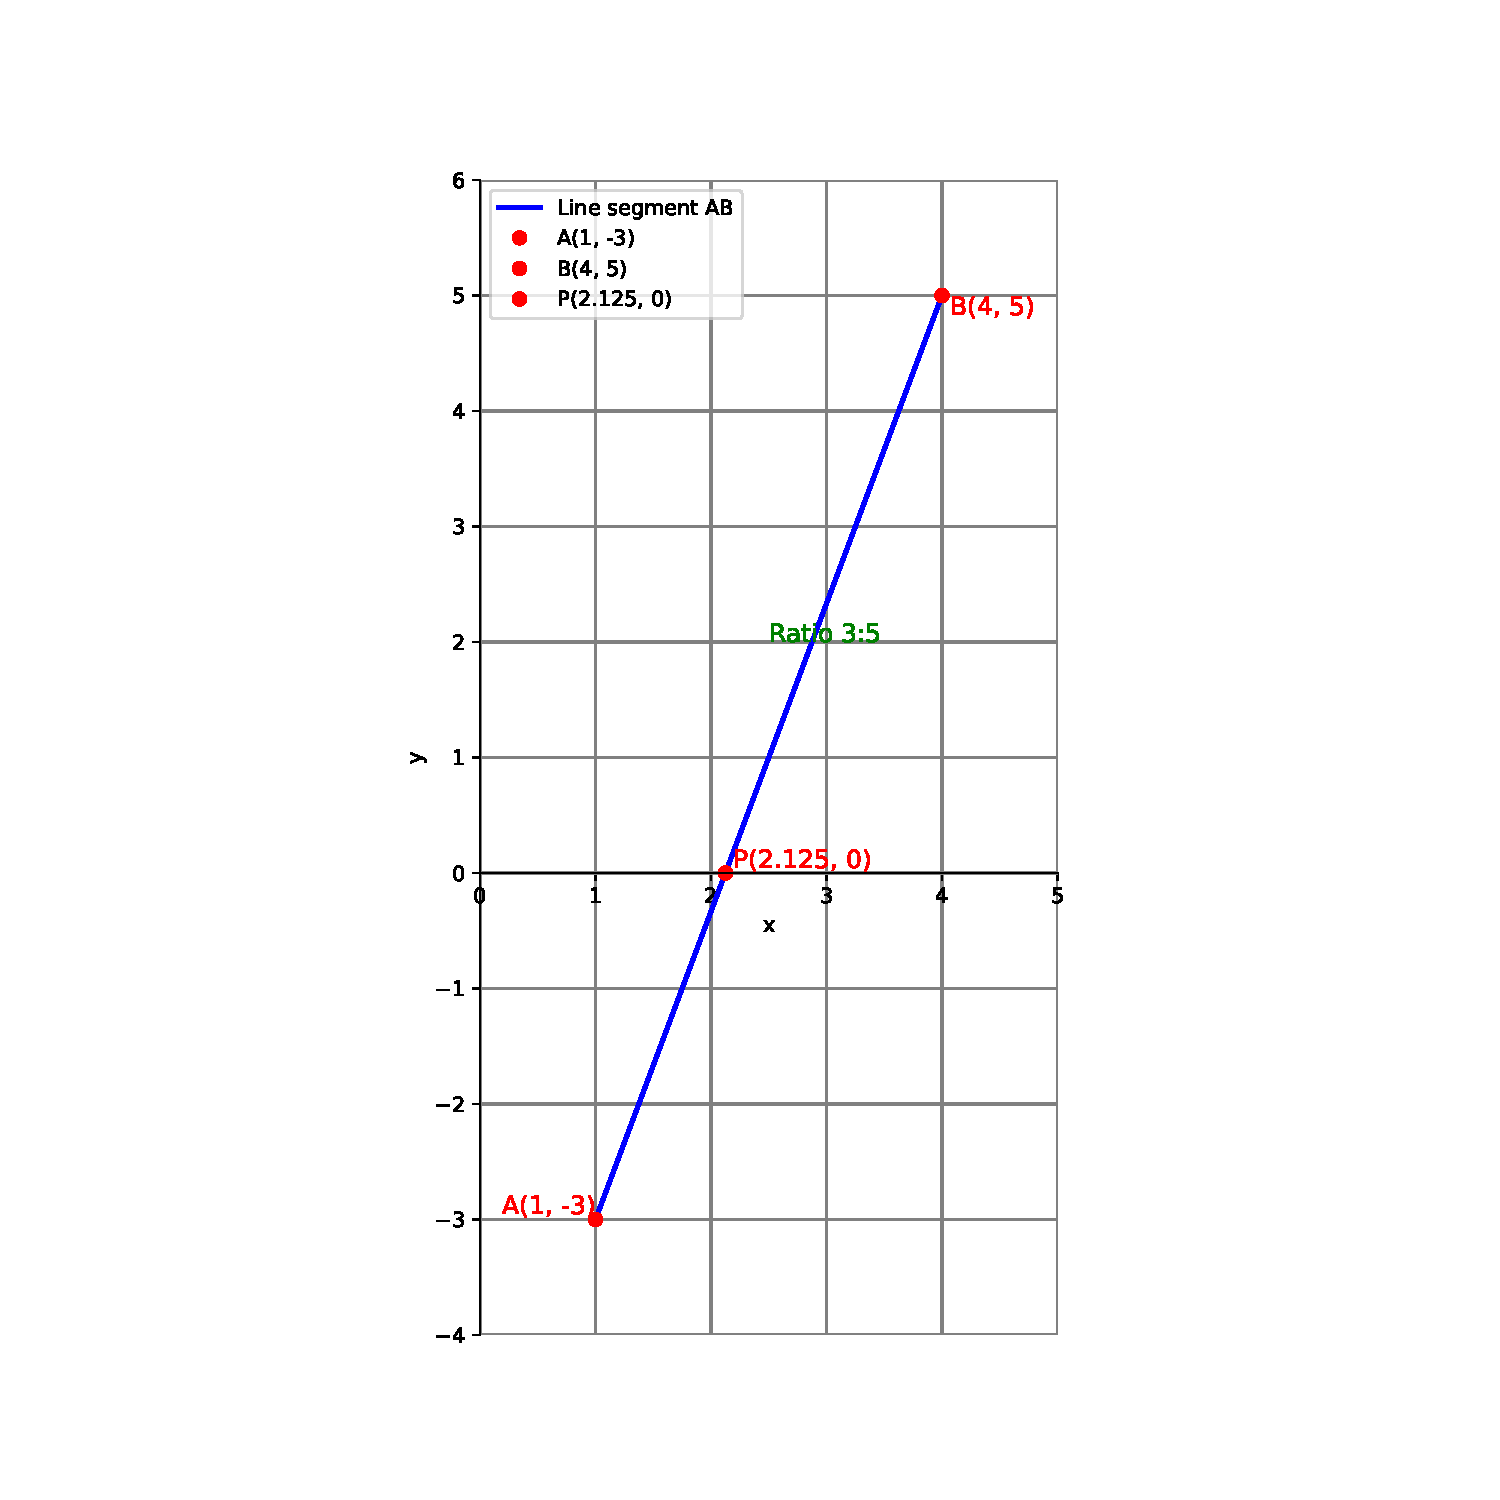
\includegraphics[width=\textwidth]{/home/tanishq/EE1030/Question1/codes/figs/line_segment_AB.pdf}
    \caption{Line Segment AB}
    \label{fig:line_segment_AB}
\end{figure}


Equation of line segment joining $A =\myvec{1 \\ -3}$ and $B= \myvec{4 \\ 5}$ given by

   $$\frac{x-1}{3}=\frac{y+3}{8}$$

   The intersection with the $x$-axis occurs when $y=0$. Substitute $y=0$ into the parametric equation:

   $$\frac{x-1}{3}=\frac{3}{8}$$

   $$x-1=\frac{3 \cdot 3}{8}=\frac{9}{8}$$

   $$x=1+\frac{9}{8}=\frac{8+9}{8}=\frac{17}{8}$$

   Therefore, the point of intersection with the $x$-axis is $\myvec{\frac{17}{8} \\ 0}$.

   Let this point $\myvec{\frac{17}{8} \\ 0 } $ divide the segment $AB$ in the ratio $k:1$. 
   
   Using section formula, 

   $$\myvec{\frac{k \cdot 4+1}{k+1} \\ \frac{k \cdot 5-3}{k+1}}=\myvec{\frac{17}{8} \\ 0 }$$

   $$ \frac{\myvec{4 \\ 5}k + \myvec{1 \\ -3 }}{k+1} = \myvec{\frac{17}{8} \\ 0 }$$

   $$ \myvec{\frac{15}{8} \\ 5 }k = \myvec{\frac{9}{8} \\ 3}   $$

   $$ \text{or}, k=\frac{3}{5} $$
   Hence, the ratio in which the line segment joining the points $A =\begin{pmatrix} 1 \\ -3 \end{pmatrix}$ and $B=\begin{pmatrix} 4 \\ 5 \end{pmatrix}$ is divided by the $x$-axis is $3:5$.
\end{document}
